\section{Results}\label{sec:results}
The original rules for the mafia game excluded roles altogether, instead
preferring the simplest version of the game consisting of two teams, the mafia
and the town. Using these rules\cite{MafiaRules}, it was recommended to have 1
mafia member per. 3 players, leading to a game setup of 3 mafia members and 7
town members. The use of this game setup in our simulation leads to the mafia
having a clear advantage, as can be seen on figure \ref{fig:VariousSimulations}
(MMGS \& MMGSD)\footnote{MMGS Refers to Mafioso, Mafioso, Godfather, Sheriff,
    and Doctor, as a role abbreviation, others can be found in \ref{app:roles}}.
The is likely due to the expanded elimination capabilities in the form of the
mafioso and the godfather. \\ Should one instead reduce the number of mafia
members to 2, and as a result increase the number of town members to 8, the
win-rates for the two teams equalize significantly more, but still being to the
mafias favour (MGSD \& MGS).\\ Getting to the subject of this report: How a
mafia fares against a powerful town\footnote{A powerful town being defined as
    one that uses all roles from appendix \ref{app:A}.}, one can look at all of the
columns after the "Powerful Town" label on the figure
(\ref{fig:VariousSimulations}). The only consistent feature of the mafia teams
represented by these columns are the presence of 1 godfather on each team. They
display that, against a powerful town, many configurations of mafia-roles are
quite balanced, resulting in mostly a 50/50 win-rate for each team. The main
exceptions for this is elimination-heavy compositions the most significant of
which being MMG, with a win-rate of 74\% for the mafia. Furthermore, it seems
that one of the only roles that can somewhat replace a mafioso in mixed-roles
compositions is the consigliere, as such compositions (CgCtG \& CgBG) fare
comparably to ones including a mafioso. \\ Below are all of the results:
\begin{figure}[H]
    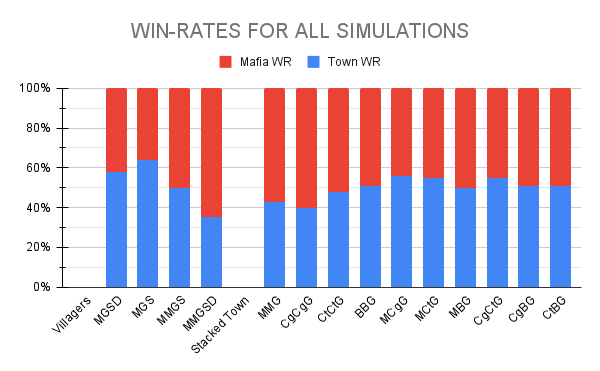
\includegraphics[width=1\linewidth]{figures/Winrates}
    \caption{\\Graph of the win-rate of various simulated game compositions.\\
        There were 10 players in each simulation.\\
        Each simulation was 100 games.
        Simulation names are related to team composition, based on role
        abbreviations in appendix \ref{app:A}.\\
        The first 4 runs labelled \textit{Villagers} means that all roles not
        mentioned in the abbreviation are replaced with villagers.\\
        The next runs labelled \textit{Powerful Town} means that all roles not
        mentioned in the abbreviation are replaced with	one of each town role.}
    \label{fig:VariousSimulations}
\end{figure}
\todo{Too much text in the caption}
\vspace{-5px}Based on this graph we can deduce that mafiosi and
consiglieri are moreto
impactful for the mafia than both consorts and blackmailers. But it also seems
that the varied team consisting of one mafioso, consigliere, and godfather,
performs marginally better than other mixed configurations. \\
The results indicate \todo{Refer to where this indicates this} that when playing against a powerful town, it is more
important for the mafia to be able to continually eliminate town members, and to be
able to quickly find the most powerful roles of the town, in order to eliminate
them, than it is to deny actions and communication to the town. \\
It would be interesting to see which of the non-eliminating mafia roles perform
best when they are on their own, and which composition of them performs best.
This type of game removes the mafias ability to eliminate during the night, while
they retain their knowledge of one another and their respective abilities to
gain information, limit nightly actions, and limit communicative actions. Figure \ref{fig:VariousSimulationsNonKilling} shows
are the results of such games:
\begin{figure}[H]
    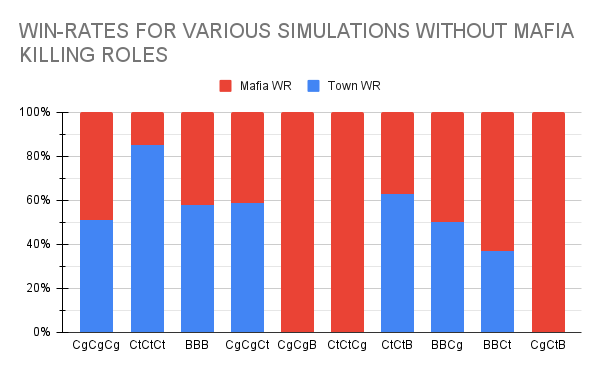
\includegraphics[width=1\linewidth]{figures/Winrates_NonKilling}
    \caption{\\Graph of the win-rate of various simulated game compositions
        with only non-eliminating mafia roles.\\
        There were 10 players in each simulation.\\
        Each simulation was 100 games.
        Simulation names are related to team composition, based on role
        abbreviations in appendix \ref{app:A}.\\
        All of the runs were against the previously explained powerful town.}
    \label{fig:VariousSimulationsNonKilling}
\end{figure}
\vspace{-5px} As seen on the above graph we can once again conclude that
consiglieri are more impactful than either consorts or blackmailers \ref{fig:VariousSimulationsNonKilling}. This may
be due to their superior abilities in finding the sheriff, enabling them to
collectively vote them out. It also seems that no mixed-combination of
non-killing mafia roles can compete with the pure-consiglieri team, except for BBCg.
